%%% https://tex.stackexchange.com/questions/85759/tikz-pgf-how-to-draw-a-node-as-a-line-rectangle-with-zero-height
%%% https://tex.stackexchange.com/questions/300702/how-to-change-arrowhead-size-and-scale-in-tikz

\documentclass{standalone}


\usepackage{tikz}
\usetikzlibrary{shapes.geometric, arrows}
\usetikzlibrary{positioning}


\tikzstyle{startstop} = [rectangle, rounded corners, minimum width=2cm, minimum
height=0.5cm,text centered, draw=black]

\tikzstyle{io} = [trapezium, trapezium left angle=70, trapezium right angle=110, minimum
width=2.5cm, minimum height=0.5cm, text centered, text width = 1.5cm, draw=black]

\tikzstyle{process} = [rectangle, minimum width=2cm, minimum height=0.5cm, text centered,
text width = 1cm, draw=black]
\tikzstyle{decision} = [diamond, minimum width=2cm, minimum height=0.5cm, text centered,
draw=black]

\tikzstyle{block1} = [rectangle, rounded corners, minimum width=0.5cm, minimum
height=0.25cm,text centered, draw=black]

\tikzstyle{block2} = [rectangle, rounded corners, minimum width=2.5cm, minimum
height=3.6cm,text centered, draw=black]



\tikzstyle{arrow} = [thick,->,>=stealth]


\usetikzlibrary{arrows.meta}

\begin{document}
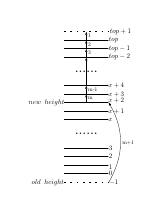
\begin{tikzpicture}[node distance=.1cm, thick]
  \tikzstyle{st2}=[rectangle, inner sep=0pt, minimum height=0pt, minimum width=16pt, draw,
  line width=0.025em]
  
  \node (h0) [st2, label={[anchor=east, inner sep=1.5pt, scale=.25,
    xshift=.25cm]east:$0$}]{};
  \node (-h) [st2, dotted, below=of h0, label={[anchor=east, inner sep=1.5pt, scale=.25,
    xshift=.55cm]east:$-1$}, label={[anchor=west, inner sep=1.5pt, scale=.25,
    xshift=-1.7cm]west:$old \enspace height$}]{};
  \node (h1) [st2, above=of h0, label={[anchor=east, inner sep=1.5pt, scale=.25,
    xshift=.25cm, yshift=-.1cm]east:$1$}]{};
  \node (h2) [st2, above=of h1, label={[anchor=east, inner sep=1.5pt, scale=.25, xshift=.25cm]east:$2$}]{};
  \node (h3) [st2, above=of h2, label={[anchor=east, inner sep=1.5pt, scale=.25, xshift=.25cm]east:$3$}]{};
  \node (more1) [above=of h3, scale=.5]{......};
  \node (x) [st2, above=of more1, label={[anchor=east, inner sep=1.5pt, scale=.25, xshift=.25cm]east:$x$}]{};
  \node (x+1) [st2, above=of x, label={[anchor=east, inner sep=1.5pt, scale=.25, xshift=.85cm]east:$x+1$}]{};
  \node (x+2) [st2, above=of x+1, label={[anchor=east, inner sep=1.5pt, scale=.25,
    xshift=.85cm, yshift=.1cm]east:$x+2$}, label={[anchor=west, inner sep=1.5pt, scale=.25,
    xshift=-1.85cm]west:$new \enspace height$}]{};
  \node (x+3) [st2, above=of x+2, label={[anchor=east, inner sep=1.5pt, scale=.25,
    xshift=.85cm]east:$x+3$}]{};
  \node (x+4) [st2, above=of x+3, label={[anchor=east, inner sep=1.5pt, scale=.25,
    xshift=.85cm]east:$x+4$}]{};
  \node (more2) [above=of x+4, scale=.5]{......};
  \node (top-2) [st2, above=of more2, label={[anchor=east, inner sep=1.5pt, scale=.25,
    xshift=1.15cm]east:$top-2$}]{};
  \node (top-1) [st2, above=of top-2, label={[anchor=east, inner sep=1.5pt, scale=.25,
    xshift=1.15cm]east:$top-1$}]{};
  \node (top) [st2, above=of top-1, label={[anchor=east, inner sep=1.5pt, scale=.25,
    xshift=.55cm]east:$top$}]{};
  \node (top+1) [st2, dotted, above=of top, label={[anchor=east, inner sep=1.5pt, scale=.25,
    xshift=1.2cm]east:$top+1$}]{};
  

  \draw[arrow, line width=0.01em, >={Stealth[inset=0pt,length=1pt]}] (top)
  -- node[right, scale=.2] {1} (top+1);
  \draw[arrow, line width=0.01em, >={Stealth[inset=0pt,length=1pt]}] (top-1)
  -- node[right, scale=.2] {2} (top);
  \draw[arrow, line width=0.01em, >={Stealth[inset=0pt,length=1pt]}] (top-2)
  -- node[right, scale=.2] {3} (top-1);
  \draw[arrow, line width=0.01em, >={Stealth[inset=0pt,length=1pt]}] (x+4)
  --  (top-2);

  \draw[arrow, line width=0.01em, >={Stealth[inset=0pt,length=1pt]}] (x+3)
  -- node[right, scale=.2] {m-1} (x+4);
  \draw[arrow, line width=0.01em, >={Stealth[inset=0pt,length=1pt]}] (x+2)
  -- node[right, scale=.2] {m} (x+3);
  \draw[arrow, line width=0.01em, >={Stealth[inset=0pt,length=1pt]}] (-h.east) to
  [out=150,in=30, bend right] node[right, scale=.2]{m+1} (x+2.east);
  
\end{tikzpicture}
\end{document}




%%% Local Variables:
%%% mode: latex
%%% TeX-master: t
%%% End:
